\documentclass[12pt,a4paper]{article}
\usepackage[brazilian]{babel}
\usepackage[utf8]{inputenc}
\usepackage[T1]{fontenc}
\usepackage{amsmath,amssymb}
\usepackage{graphicx}
\usepackage{geometry}
\usepackage{enumitem}
\usepackage{hyperref}
\geometry{margin=2.5cm}

\title{Aula 01 - Introducao a Modelagem\\Resumo, Exemplo e Exercicios Resolvidos}
\author{Baseado apenas nos arquivos da pasta 1 - Introducao}
\date{14/04/2026}

\begin{document}
\maketitle

\section{Resumo rapido}
Pelos arquivos desta pasta (slides e tarefa), os pontos centrais sao:
\begin{itemize}
  \item modelagem matematica e computacional como processo de representar problemas reais;
  \item escolha de ferramentas computacionais conforme o problema (simulacao, linguagem, sistema);
  \item fluxo geral: problema real $\to$ modelo $\to$ simulacao $\to$ comparacao com realidade;
  \item metodos deterministicos e metodos estocasticos (Monte Carlo) como abordagens possiveis.
\end{itemize}

\section{Explicacao simples}
Este tema ensina a transformar uma pergunta real em um roteiro matematico:
\begin{enumerate}
  \item escolher o que medir (altura, velocidade, tempo);
  \item escrever as regras fisicas (equacoes);
  \item resolver e comparar com o que acontece no mundo real.
\end{enumerate}
No caso da queda livre, a ideia principal e: a gravidade muda a velocidade a cada instante.

\section{Exemplo guiado}
Problema: objeto largado de altura $H$ com velocidade inicial $v_0$.
\begin{align}
\frac{dv}{dt} &= -g, \\
\frac{dy}{dt} &= v.
\end{align}
Com $y(0)=H$ e $v(0)=v_0$, segue:
\begin{align}
v(t) &= v_0-gt, \\
y(t) &= H+v_0t-\frac{1}{2}gt^2.
\end{align}

\section{Exercicios dos slides resolvidos passo a passo}
O arquivo \textbf{Tarefa01.txt} traz uma tarefa de modelagem de queda livre. Abaixo, a resolucao de cada item.

\subsection*{1) Implementar modelo de queda livre com altura inicial $H$ e velocidade $v_0$}
Modelo sem resistencia do ar:
\begin{align}
\frac{dv}{dt} &= -g, \\
\frac{dy}{dt} &= v,
\end{align}
com condicoes iniciais $y(0)=H$ e $v(0)=v_0$.

Solucao analitica:
\begin{align}
v(t) &= v_0 - gt, \\
y(t) &= H + v_0 t - \frac{1}{2}gt^2.
\end{align}

Tempo de impacto (quando $y(t_*)=0$):
\begin{equation}
t_* = \frac{v_0 + \sqrt{v_0^2 + 2gH}}{g}.
\end{equation}

\subsection*{2) Graficos de posicao, velocidade e aceleracao}
Do modelo:
\begin{itemize}
  \item posicao: parabola concava para baixo;
  \item velocidade: reta decrescente no tempo;
  \item aceleracao: constante, $a(t)=-g$.
\end{itemize}

\begin{figure}[htbp]
\centering
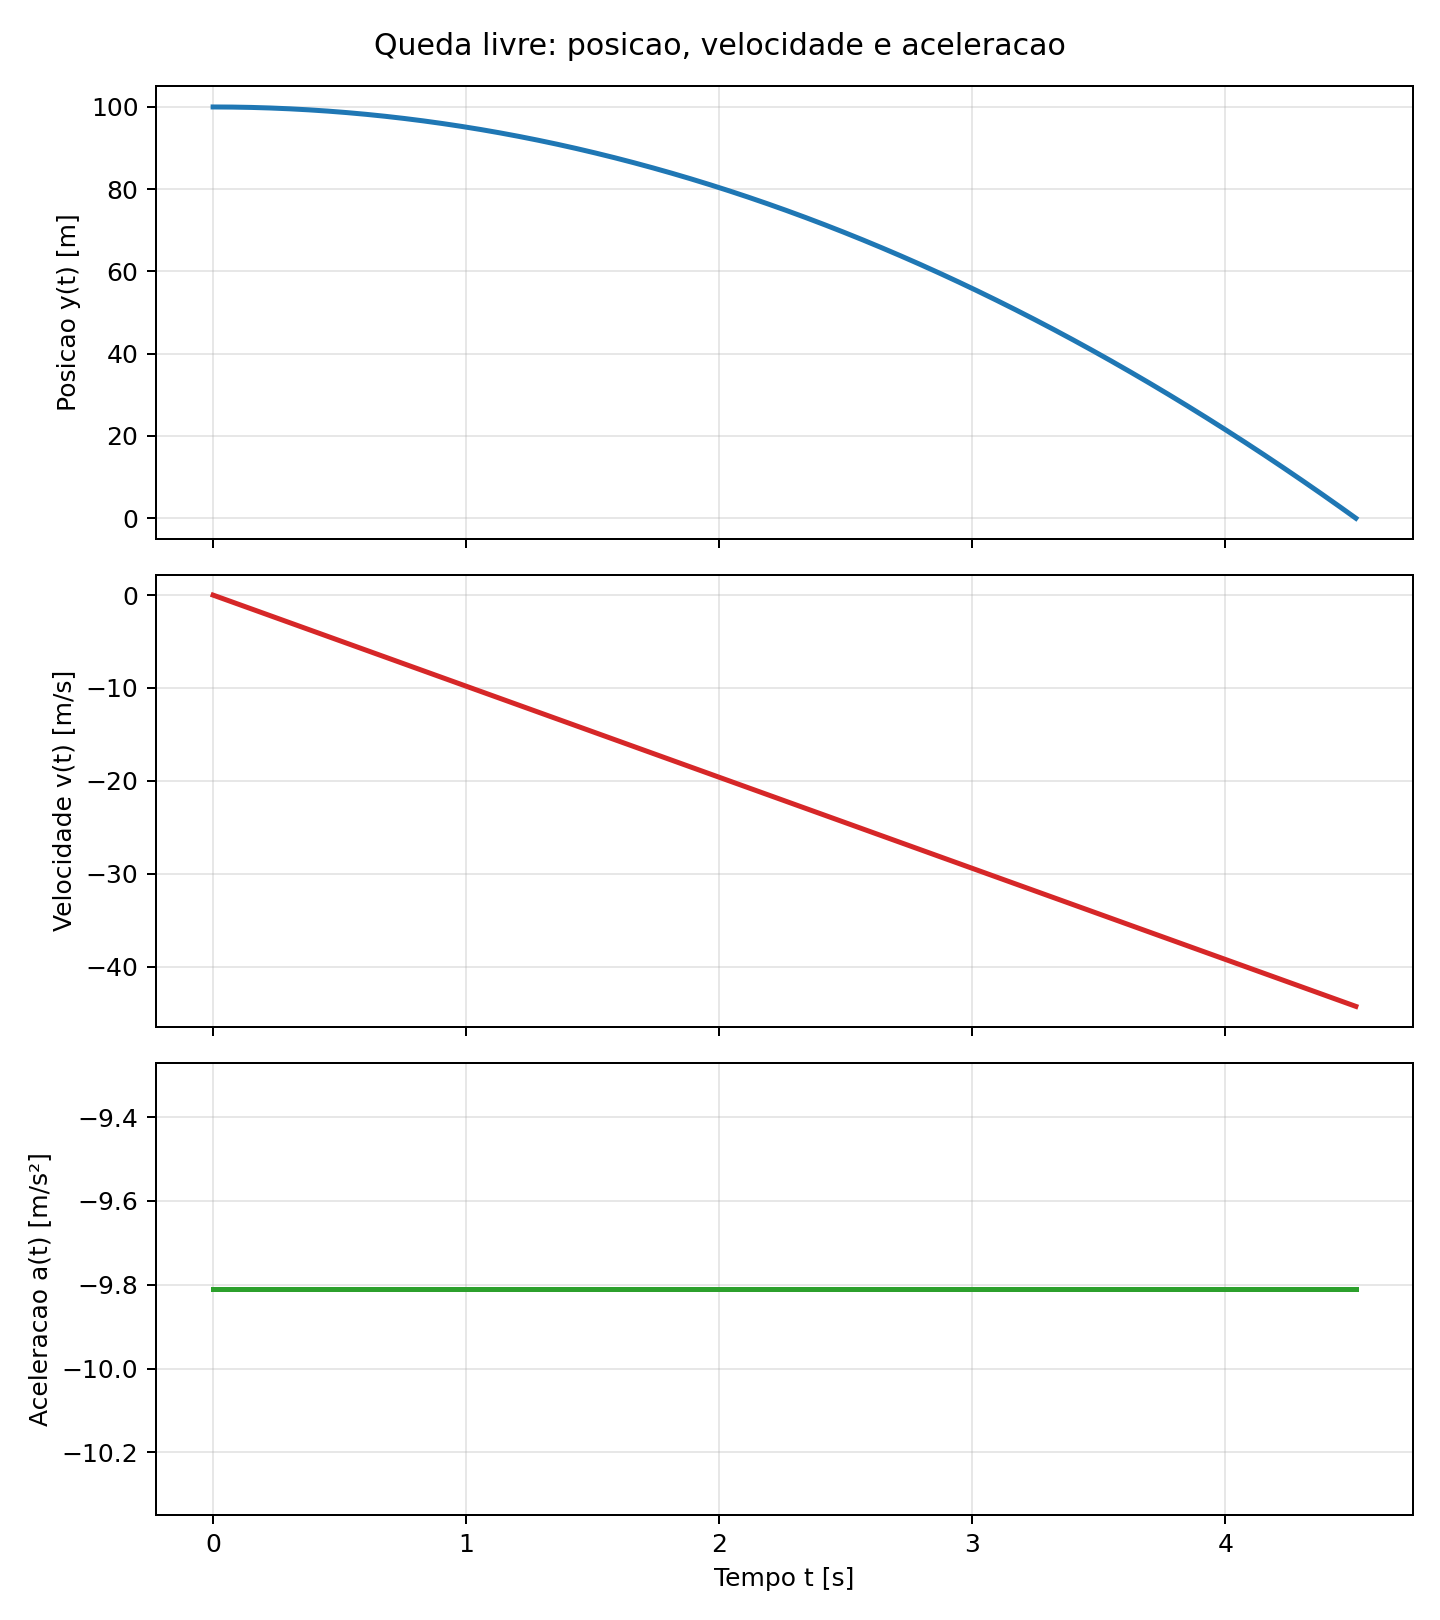
\includegraphics[width=0.9\textwidth]{figuras/queda_livre_curvas.png}
\caption{Representacao grafica da queda livre do Exercicio 2.}
\end{figure}

\subsection*{3) Quais mudancas se for corpo rigido?}
Para corpo rigido, surgem efeitos nao presentes no ponto material:
\begin{itemize}
  \item rotacao (momento de inercia, torque aerodinamico);
  \item orientacao do corpo altera area frontal e coeficiente de arrasto;
  \item possivel acoplamento translacao-rotacao.
\end{itemize}
Assim, o sistema passa a exigir equacoes adicionais para variaveis angulares.

\subsection*{4) Resistencia do ar (extra)}
Modelo com arrasto linear:
\begin{equation}
\frac{dv}{dt} = -g - kv.
\end{equation}
Solucao para $v(0)=v_0$:
\begin{equation}
v(t)=\left(v_0+\frac{g}{k}\right)e^{-kt}-\frac{g}{k}.
\end{equation}
A velocidade terminal e:
\begin{equation}
v_{term}=-\frac{g}{k}.
\end{equation}

\subsection*{5) Acuracia em funcao do passo de tempo (extra)}
Usando Euler explicito:
\begin{align}
v_{n+1} &= v_n - g\,\Delta t, \\
y_{n+1} &= y_n + v_n\,\Delta t.
\end{align}
O erro global do Euler e de ordem $\mathcal{O}(\Delta t)$.
Portanto, reduzir $\Delta t$ melhora a acuracia aproximadamente de forma linear.

\section{Fontes web para revisar}
\begin{itemize}
  \item Modelagem matematica (visao geral): \url{https://pt.wikipedia.org/wiki/Modelagem_matem%C3%A1tica}
\end{itemize}

\end{document}
